\section*{Dataset validation}
%Use section and subsection commands to organize your document. \LaTeX{}
%handles all the formatting and numbering automatically. Use ref and label
%commands for cross-references.

%This section is not essential for Web Tool papers. 
%For Data Articles, no analysis of the data, results or conclusions should be
%included and so this section should not be completed. 

\textit{This is currently just a dump of some descriptive statistics.}

Annotations for a total of \AVTotalCharLabels\ and \AOTotalCharLabels\
different characters were created for the audio-visual movie (AV) and the audio
movie (AO) respectively. There are \AVThreshCharLabels~(AV) and
\AOThreshCharLabels~(AO) characters for which there is a \AVAggThresh\ minimum
inter-rater agreement on the presence of a portrayed emotion for at least five
episodes of one second or longer throughout the entire movie. The number of
emotion episodes for for these characters is shown in figure \ref{fig:threshchar}.
As expected, the majority of all portrayed emotions are associated with the main
movie characters Forrest, Dan, and Jenny.

\begin{figure}
  \centering
  \includegraphics[width=\linewidth]{figures/character_episodes}
  \caption{Portrayed emotion by movie character. Only characters with five or
    more episodes of portrayed emotions are shown. All considered episodes for a particular character
    show a minimum inter-rater agreement of \AVAggThresh\ with respect to their
    presence at a particular time in the movie, not necessarily in terms of the
    nature of the emotion. (A) Number of episodes
    per character for both movie variants. (B) Total duration of emotion display
    across all considered episodes.}
  \label{fig:threshchar}
\end{figure}

For the audio movie \AOFracWithLabeledEmotions\ of all annotations include at
least one of the 22 explicit emotion label (see table
\ref{tab:emotion_categories}, whereas only \AVFracWithLabeledEmotions\ of
annotations for the audio-visual movie contain such a label. This is an
indication that emotion cues in the visual movie more diverse and ambiguous in
comparison to the audio-only stimulus. Figure \ref{fig:threshlabeledemotion}
shows the frequency of individual emotion. For both stimulus types the majority
of all emotional episodes involve the five categories anger/rage, fear,
happiness, love and sadness.

\begin{figure}
  \centering
  \includegraphics[width=\linewidth]{figures/labeledemotion_episodes}
  \caption{Episodes of portrayed emotion by category. Only observations assigning
    one of the 22 emotion labels were considered, and only emotion categories
    with five or more episodes are shown. All considered episodes for a particular emotion
    show a minimum inter-rater agreement of \AVAggThresh\ with respect to their
    presence at a particular time in the movie, not necessarily in terms of the
    portraying character. (A) Number of episodes
    per emotion category for both movie variants. (B) Total duration of emotion
    display across all considered episodes.}
  \label{fig:threshlabeledemotion}
\end{figure}

Almost all annotations (AO: \AOFracWithLabeledOncue; AV:
\AVFracWithLabeledOncue) include information on the nature of the cue(s)
indicating the onset or presence of an emotion. Only considering annotations
with a minimum inter-rater agreement of \AVAggThresh\ with respect to the type
of onset cue, the two dominating emotion cues are mimic/facial expressions
(only for the audio-visual movie) and verbal cues (for both stimulus types)
Figure \ref{fig:threshlabeledoncue} shows the frequency of individual emotion
onset cues for all six distinguished cue types.


\begin{figure}
  \centering
  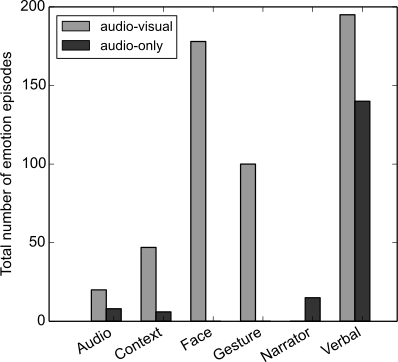
\includegraphics[width=\linewidth]{figures/labeledoncue_episodes}
  \caption{Number of emotion episodes for all distinguished onset cue categories
    (minimum \AVAggThresh\ inter-rater agreement) for both stimulus types.}
  \label{fig:threshlabeledoncue}
\end{figure}
